% Options for packages loaded elsewhere
\PassOptionsToPackage{unicode}{hyperref}
\PassOptionsToPackage{hyphens}{url}
%
\documentclass[
]{article}
\usepackage{lmodern}
\usepackage{amsmath}
\usepackage{ifxetex,ifluatex}
\ifnum 0\ifxetex 1\fi\ifluatex 1\fi=0 % if pdftex
  \usepackage[T1]{fontenc}
  \usepackage[utf8]{inputenc}
  \usepackage{textcomp} % provide euro and other symbols
  \usepackage{amssymb}
\else % if luatex or xetex
  \usepackage{unicode-math}
  \defaultfontfeatures{Scale=MatchLowercase}
  \defaultfontfeatures[\rmfamily]{Ligatures=TeX,Scale=1}
\fi
% Use upquote if available, for straight quotes in verbatim environments
\IfFileExists{upquote.sty}{\usepackage{upquote}}{}
\IfFileExists{microtype.sty}{% use microtype if available
  \usepackage[]{microtype}
  \UseMicrotypeSet[protrusion]{basicmath} % disable protrusion for tt fonts
}{}
\makeatletter
\@ifundefined{KOMAClassName}{% if non-KOMA class
  \IfFileExists{parskip.sty}{%
    \usepackage{parskip}
  }{% else
    \setlength{\parindent}{0pt}
    \setlength{\parskip}{6pt plus 2pt minus 1pt}}
}{% if KOMA class
  \KOMAoptions{parskip=half}}
\makeatother
\usepackage{xcolor}
\IfFileExists{xurl.sty}{\usepackage{xurl}}{} % add URL line breaks if available
\IfFileExists{bookmark.sty}{\usepackage{bookmark}}{\usepackage{hyperref}}
\hypersetup{
  pdftitle={DGPuK-Stellenmonitoring 2020},
  pdfauthor={Julia Niemann-Lenz \& Manuel Menke},
  hidelinks,
  pdfcreator={LaTeX via pandoc}}
\urlstyle{same} % disable monospaced font for URLs
\usepackage{longtable,booktabs}
\usepackage{calc} % for calculating minipage widths
% Correct order of tables after \paragraph or \subparagraph
\usepackage{etoolbox}
\makeatletter
\patchcmd\longtable{\par}{\if@noskipsec\mbox{}\fi\par}{}{}
\makeatother
% Allow footnotes in longtable head/foot
\IfFileExists{footnotehyper.sty}{\usepackage{footnotehyper}}{\usepackage{footnote}}
\makesavenoteenv{longtable}
\usepackage{graphicx}
\makeatletter
\def\maxwidth{\ifdim\Gin@nat@width>\linewidth\linewidth\else\Gin@nat@width\fi}
\def\maxheight{\ifdim\Gin@nat@height>\textheight\textheight\else\Gin@nat@height\fi}
\makeatother
% Scale images if necessary, so that they will not overflow the page
% margins by default, and it is still possible to overwrite the defaults
% using explicit options in \includegraphics[width, height, ...]{}
\setkeys{Gin}{width=\maxwidth,height=\maxheight,keepaspectratio}
% Set default figure placement to htbp
\makeatletter
\def\fps@figure{htbp}
\makeatother
\setlength{\emergencystretch}{3em} % prevent overfull lines
\providecommand{\tightlist}{%
  \setlength{\itemsep}{0pt}\setlength{\parskip}{0pt}}
\setcounter{secnumdepth}{5}
\usepackage{booktabs}
\usepackage{flafter}
\usepackage{booktabs}
\usepackage{longtable}
\usepackage{array}
\usepackage{multirow}
\usepackage{wrapfig}
\usepackage{float}
\usepackage{colortbl}
\usepackage{pdflscape}
\usepackage{tabu}
\usepackage{threeparttable}
\usepackage{threeparttablex}
\usepackage[normalem]{ulem}
\usepackage{makecell}
\usepackage{xcolor}
\ifluatex
  \usepackage{selnolig}  % disable illegal ligatures
\fi
\usepackage[]{natbib}
\bibliographystyle{apalike}

\title{DGPuK-Stellenmonitoring 2020}
\author{Julia Niemann-Lenz \& Manuel Menke}
\date{2021-08-05}

\begin{document}
\maketitle

{
\setcounter{tocdepth}{2}
\tableofcontents
}
\newpage

\hypertarget{vorwort}{%
\section*{Vorwort}\label{vorwort}}
\addcontentsline{toc}{section}{Vorwort}

Die Diskussion über faire Arbeitsbedingungen in der Wissenschaft ist ein Dauerthema der Arbeit der Mitelbauvertreter:innen. Bislang existierte kein Überblick über den Stellenmarkt der Kommunikations- und Medienwissenschaft im deutschsprachigen Raum. Es fehlten sowohl Erkenntnisse über die Anzahl der für unser Fach ausgeschriebenen Stellen, noch über deren konkrete Ausgestaltung.

Ein solcher Überblick ist vor dem Hintergrund der üblichen Befristung der meisten Arbeitsplätze im Wissenschaftssystem, der damit verbundenen hohen Fluktuation der Personen auf den jeweiligen Stellen und der Prekarisierung des wissenschaftlichen Mittelbaus notwendig und wurde von den DGPuK-Mittelbauvertreter:innen seit langem angestrebt. Relevant ist dies nicht nur als Orientierungshilfe für (zukünftige) Doktorand:innen und Postdocs, sondern auch als eine dauerhaft angelegte Standortbestimmung eines sich rasant wandelnden und professionalisierenden Fachs.
Nach dem Vorbild der Deutschen Vereinigung für Politische Wissenschaft (DVPW), die seit 2011 ein regelmäßiges Stellenmonitoring durchführt, wurde als Pilotprojekt die Codierung der Stellenanzeigen die im Jahr 2020 auf der Website der DGPuK veröffentlicht wurden, durchgeführt.

Wir wünschen Euch und Ihnen viel Spaß bei der Lektüre,

Julia Niemann-Lenz \& Manuel Menke

\newpage

\hypertarget{codierung}{%
\section{Codierung}\label{codierung}}

Die Genese des ``Stellenmonitorings für die DGPuK'' ist lang. Zum ersten Mal wurde das Projekt auf dem zweiten ``Nachwuchstag der DGPuK'' 2014 in Berlin angedacht. Es folgte die Entwicklung eines ausführlichen Codebuchs und endlich 2019, der erste Pretest mit drei Codierer:innen an der HMTM Hannover. Der Pretest fiel in großen Teilen zufriedenstellend aus. Bei den Variablen, die eine geringe Intercoder-Relaibilität (Krippendorff´s Alpha \textless{} .7) aufwiesen wurden nachgebessert, indem die Codieranweisungen präzisiert und das Codebuch umstrukturiert wurde. Dies betrifft insbesondere den Bereich der Aufgaben und Anforderungen an den Bewerbenden. Zudem wurde das Codebuch deutlich gekürzt, um es handhabbarer zu machen. Das aktuelle Codebuch kann \href{data/Konzept_Stellenmonitoring_2021-08-05.pdf}{hier} heruntergeladen werden.

Die Codierung der Stellenanzeigen aus 2020 erfolgte im Frühjahr und Sommer 2021 durch eine Honorarkraft, die von der DGPuK finanziert wurde. Insgesamt wurden im Erhebungszeitraum 141 Stellenanzeigen auf der \href{https://www.dgpuk.de/de/stellenangebote.html}{DGPuK-Website} veröffentlicht, die alle codiert wurden.

\hypertarget{allgemeines}{%
\section{Allgemeines}\label{allgemeines}}

\hypertarget{land-und-hochschule-der-ausschreibung}{%
\subsection{Land und Hochschule der Ausschreibung}\label{land-und-hochschule-der-ausschreibung}}

Im Rahmen der Codierung wurde zunächst geprüft, aus welchem Land die Stellenanzeigen stammen. Wenig überraschend macht dabei Deutschland mit 77\% den größten Anteil aus. Aus Österreich stammen 13\% Stellen und aus der Schweiz 8\%. Die restlichen n = 3 kommen aus dem europäischen Ausland (Norwegen, Belgien).

In Tabelle \ref{tab:pospercountry} sind die ausgeschriebenen Positionen nach Land der Ausschreibung aufgeschlüßelt.

\begin{table}[H]

\caption{\label{tab:pospercountry}Position nach Land}
\centering
\begin{tabular}[t]{l|r|r|r|r}
\hline
Position & Deutschland & Österreich & Schweiz & Sonstiges\\
\hline
WiMi allgemein (unklar/egal) & 8 & 0 & 0 & 0\\
\hline
WiMi PräDoc & 49 & 8 & 9 & 1\\
\hline
WiMi PostDoc & 21 & 5 & 2 & 0\\
\hline
WiMi LbA & 3 & 0 & 0 & 0\\
\hline
Professur (allgemein) & 4 & 5 & 0 & 2\\
\hline
W1-Professur & 5 & 0 & 0 & 0\\
\hline
W2-Professur & 12 & 0 & 0 & 0\\
\hline
W3-Professur & 3 & 0 & 0 & 0\\
\hline
Sonstige Ausschreibung & 3 & 1 & 0 & 0\\
\hline
Total & 108 & 19 & 11 & 3\\
\hline
\end{tabular}
\end{table}

In Tabelle \ref{tab:institutions} sind die Hochschulen mit fünf oder mehr Ausschreibungen im Sample aufgelistet. Insbesondere die Universität Wien sticht mit 12 Anzeigen deutlich hervor.

\begin{table}[H]

\caption{\label{tab:institutions}Hochschulen mit drei oder mehr Ausschreibungen im Sample}
\centering
\begin{tabular}[t]{l|r}
\hline
Ausschreibende Hochschule & n\\
\hline
Universität Wien & 12\\
\hline
Universität Passau & 8\\
\hline
Freie Universität Berlin & 7\\
\hline
LMU München & 7\\
\hline
Universität Hamburg & 7\\
\hline
Universität Zürich & 7\\
\hline
\end{tabular}
\end{table}

Die geografische Verteilung der Stellenanzeigen ist in Abbildung \ref{fig:germanmap} dargestellt.

\begin{figure}
\centering
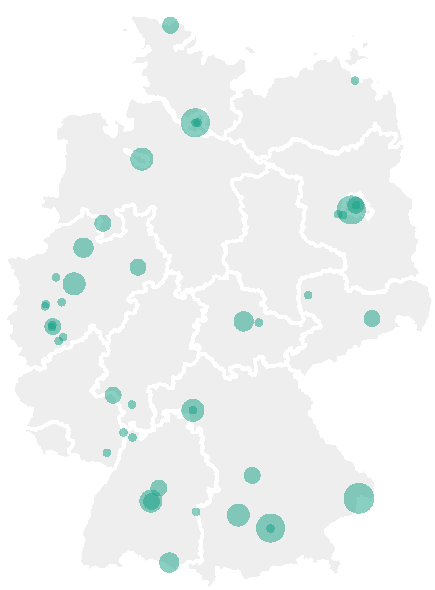
\includegraphics{dgpuksm_files/figure-latex/germanmap-1.pdf}
\caption{\label{fig:germanmap}Stellenanzeigen nach Standort (nur Deutschland)}
\end{figure}

\hypertarget{fristen-zur-bewerbung-besetzung}{%
\subsection{Fristen zur Bewerbung \& Besetzung}\label{fristen-zur-bewerbung-besetzung}}

Die Zeitspanne zwischen Ausschreibung und Deadline der Bewerbung beträgt im Mittel \emph{M} = 52 Tage (\emph{SD} = 71. Allerdings fließen nur n = 17 Fälle in diese Analyse ein, weil das Datum der Veröffentlichung der Stellenangebote sehr oft unbekannt ist (Minimum: 9, Maximum: 303).

Etwas mehr Daten liegen zur vorgesehen Dauer des Sichtungs- und Einstellungsprozesses vor, denn Angaben zum gewünschten Starttermin des Anstellungsverhältnisses finden sich fast immer. In vielen Fällen (n = 50) soll die Einstellung ``asap'' (as soon as possible) erfolgen. Die mittlere Dauer zwischen Ende der Deadline und Beginn der Anstellung lässt sich jedoch nur berechnen, wenn beide Daten ermittelt werden konnten. Dies gilt für n = 77 Anzeigen. Die Mittlere Dauer beträgt \emph{M} = 88 (\emph{SD} = 65) (Minimum: 12, Maximum: 374).

Für die Besetzung von Professuren wird sich naturgemäß wegen des aufwändigen Berufungsprozesses im Mittel deutlich mehr Zeit gelassen als für Wissenschaftliche Mitarbeiterinnen (Tabelle \ref{tab:timeperposition}).

\begin{table}[H]

\caption{\label{tab:timeperposition}Durchschnittliche Dauer zwischen Deadline und Beginn der Stelle nach Position in Tagen}
\centering
\begin{tabular}[t]{l|r|r|r}
\hline
Position & M & SD & n\\
\hline
WiMi & 76 & 45 & 106\\
\hline
Professur & 194 & 121 & 31\\
\hline
\end{tabular}
\end{table}

Für Bewerber:innen ist natürlich die Frage interessant, ob der Stellenmarkt saisonal schwankt. Natürlich lässt die Betrachtung von nur einem Jahr darauf kaum Rückschlüsse zu. Es scheint aber so zu sein, dass Deadlines für die Bewerbungen eher am Anfang der oder in den Semesterferien liegen. Wie in Abbildung \ref{fig:monthly} zu sehen ist, verstrichen 2020 die meisten Bewerbungsdeadlines allerdings bereits im Januar (für diese Analyse wurden nur Stellenanzeigen betrachtet, die 2020 endeten, Januar 2021 ist nicht enthalten).

\begin{figure}
\centering
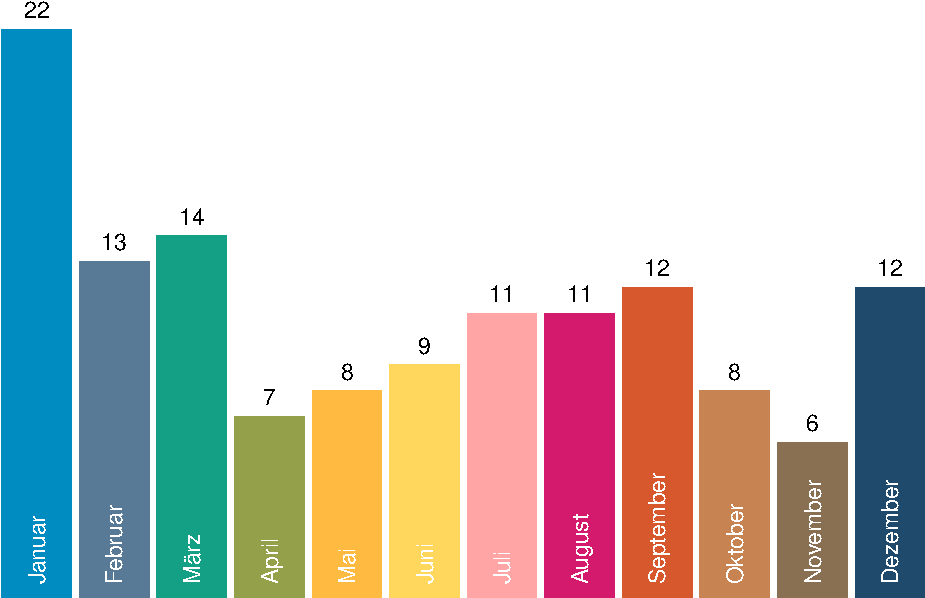
\includegraphics{dgpuksm_files/figure-latex/monthly-1.pdf}
\caption{\label{fig:monthly}Stellenanzeigen im Jahresverlauf}
\end{figure}

\hypertarget{ausgeschriebene-positionen}{%
\subsection{Ausgeschriebene Positionen}\label{ausgeschriebene-positionen}}

Die Stellenanzeigen verteilen sich wie folgt auf die verschiedenen Positionen (Tabelle \ref{tab:position}):

\begin{table}

\caption{\label{tab:position}Ausgeschriebene Positionen im Sample}
\centering
\begin{tabular}[t]{l|r|r}
\hline
Stelle & n & Prozent\\
\hline
WiMi PräDoc & 67 & 0.48\\
\hline
WiMi PostDoc & 28 & 0.20\\
\hline
W2-Professur & 12 & 0.09\\
\hline
Professur (allgemein) & 11 & 0.08\\
\hline
WiMi allgemein (unklar/egal) & 8 & 0.06\\
\hline
W1-Professur & 5 & 0.04\\
\hline
Sonstige Ausschreibung & 4 & 0.03\\
\hline
WiMi LbA & 3 & 0.02\\
\hline
W3-Professur & 3 & 0.02\\
\hline
\end{tabular}
\end{table}

Bei den ``sonstigen'' Stellen handelt es sich um Stipendien, Gastprofessuren oder Honorarauftäge (für Forschung oder Lehre). Sie werden im Folgenden nicht weiter berücksichtigt.

\hypertarget{angaben-zu-gleichstellung-behinderung-und-familienfreundlichkeit-etc.}{%
\subsection{Angaben zu Gleichstellung, Behinderung und Familienfreundlichkeit etc.}\label{angaben-zu-gleichstellung-behinderung-und-familienfreundlichkeit-etc.}}

Viele Stellenangebote enthalten Angaben zur Gleichstellung, zu Bewerber:innen mit Schwerbehinderung oder Migrationshintergrund. Außerdem werben viele Hochschulen mit Familienfreundlichkeit und Dual-Career. Zudem werden bisweilen Angaben dazu gemacht, ob eine Stelle Teilzeit-fähig ist. Abbildung \ref{fig:appl} zeigt getrennt für Stellenanzeigen für Professuren bzw. WiMis auf, welche Angaben zu wieviel Prozent in den Stellenanzeigen enthalten waren.

\begin{figure}
\centering
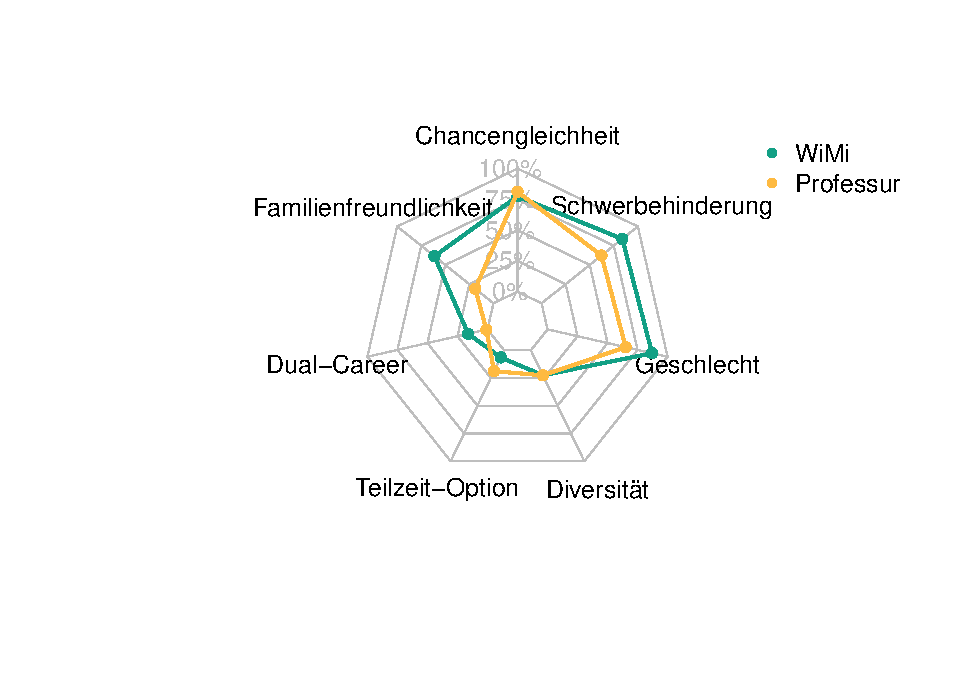
\includegraphics{dgpuksm_files/figure-latex/appl-1.pdf}
\caption{\label{fig:appl}Angaben zur Besetzung (Professur/WiMi)}
\end{figure}

Es wird offensichtlich, dass bei Professuren die Angaben zur Familienfreundlichkeit, Gleichstellung und Schwerbehinderung häufiger erwähnt werden. Explizit teilzeitfähig sind die Professuren hingegen sehr selten. Auch Dual-Career-Angebote werden kaum erwähnt. Die Möglichkeit zur Teilzeitarbeit wird hingegen bei WiMis häufiger hervorgehoben -- jedoch ebenfalls auf niedrigem Niveau. Die Stellen sind ja ohnehin zu einem großen Anteil keine vollen Stellen.

\hypertarget{angaben-zur-uxfcbernahme-von-reisekosten}{%
\subsection{Angaben zur Übernahme von Reisekosten}\label{angaben-zur-uxfcbernahme-von-reisekosten}}

Von den 141 Stellenangeboten enthielten die allermeisten (128) keine Angabe dazu, ob die Anfahrtskosten für ein Bewerbungsgespräch übernommen werden. In 11 Fällen wurde explizit darauf hingewiesen, dass die Kosten \emph{nicht} übernommen werden. Nur in 2 Fällen (= 1.4 \%) fand sich der Hinweis, dass der Arbeitgeber die Kosten der Anreise trägt.

\hypertarget{wissenschaftliche-mitarbeiterinnen}{%
\section{Wissenschaftliche Mitarbeiter:innen}\label{wissenschaftliche-mitarbeiterinnen}}

\hypertarget{land}{%
\subsection{Land}\label{land}}

\begin{table}[H]

\caption{\label{tab:unnamed-chunk-1}Wissenschaftliche Mitarbeiter nach Land}
\centering
\begin{tabular}[t]{l|r|r}
\hline
Land & n & Prozent\\
\hline
Deutschland & 81 & 0.76\\
\hline
Österreich & 13 & 0.12\\
\hline
Schweiz & 11 & 0.10\\
\hline
Sonstiges & 1 & 0.01\\
\hline
\end{tabular}
\end{table}

Die folgenden Analysen beziehen sich nur auf Deutschland.

\hypertarget{befristungen-der-wissenschaftlichen-mitarbeiterinnen}{%
\subsection{Befristungen der Wissenschaftlichen Mitarbeiter:innen}\label{befristungen-der-wissenschaftlichen-mitarbeiterinnen}}

Die Stellen für Wissenschaftliche Mitarbeiter:innen in Deutschland wurden in der Regel befristet und unter Berufung auf das WissZeitVG ausgeschrieben. Das WissZeitVG sieht nach § 2 Abs. 1 vor, dass die Befristung mit einer (angestrebten) Qualifizierung (= Promotion oder Habilitation) begründet wird. Nach § 2 Abs. 2 sind auch Befristungen möglich, wenn die Stelle aus Mitteln Dritter finanziert wird und diese Mittel zeitlich befristet sind. Tabelle \ref{tab:limits} gibt einen Überblick über Befristung vs.~Nicht-Befristung bei den WiMi-Stellen im Sample. Wenig überraschend wird deutlich, dass Stellenausschreibungen für unbefristete Stellen quasi kaum existieren.

\begin{table}[H]

\caption{\label{tab:limits}Befristungen bei Wissenschaftlichen Mitarbeiterstellen}
\centering
\begin{tabular}[t]{l|r|r}
\hline
Stelle & befristet & unbefristet\\
\hline
WiMi allgemein (unklar/egal) & 8 & 0\\
\hline
WiMi PräDoc & 49 & 0\\
\hline
WiMi PostDoc & 21 & 0\\
\hline
WiMi LbA & 2 & 1\\
\hline
\end{tabular}
\end{table}

Im ganzen Sample findet sich nur eine unbefristete Mittelbau-Stelle als \textbf{Lehrkraft für besondere Aufgaben (LbA)}. Da bei LbA-Stellen keine eigene Qualifizierung vorgesehen ist, gilt für sie keine Lehrreduzierung. Außerdem können sie in der Regel zudem nicht nach § 2 Abs. 1 WissZeitVG befristet werden (weil keine Qualifizierung vorgesehen ist). Dennoch findet sich im Sample auch eine Stelle als LbA, die ausdrücklich nach § 2 Abs. 1 WissZeitVG auf 3 Jahre befristet ist, und die 12 LVS aufweist. Eine Möglichkeit der Entfristung wird in der Stellenanzeige nicht erwähnt. Wie der/die Stelleninhaberin unter diesen Bedingungen ein Qualifizierungsziel erreichen soll, bleibt offen. Die dritte LbA-Stelle folgt anderen Befristungsregeln (außerhalb des WissZeitVG) und eine Entfristung wird angestrebt.

In 53 Prozent der befristeten Stellenangebote findet sich ein Hinweis auf die \textbf{anzustrebende Qualifikation}. Eine \textbf{strukturierte Dokorandenausbildung}, etwa im Rahmen eines PhD-Programms, wird in 18 Prozent der PräDoc-Stellen erwähnt.

Die eigene Qualifikation ist aber nicht immer der (einzige) Befristungsgrund. In 43 Prozent der Fälle findet die Beschäftigung zumindest teilweise in einem \textbf{durch Drittmittel finanzierten Projekt} statt. Dies betrifft Stellen für Promovierende geringfügig mehr als solche für Postdocs (48 gegenüber 36 Prozent), während die Stellen, bei denen die Besetzung sowohl durch eine:n Postdoc als auch ein:e Doktorand:in möglich ist, zu 38 Prozent aus Drittmitteln finanziert werden.

Die \textbf{Dauer der Befristung} für den im Stellenagebot beworbenen Vertrag beträgt zwischen 0.33 und 6 Jahren. Bei der 4-Monatsstelle handelt es sich um eine Elternzeitvertretung. Die mittlere Vertragsdauer ist \emph{M} = 3.13 Jahre (\emph{SD} = 1.13).

In einigen Stellenangeboten wird nach Ablauf des ersten Vertrages eine \textbf{Verlängerung} in Aussicht gestellt (Tabelle \ref{tab:limitextension}). Dies ist jedoch nur bei 27 Prozent der Stellenangebote für WiMis der Fall. In 2 Fällen wird sogar eine \textbf{Entfristung} des Vertrags angestrebt.

\begin{table}[H]

\caption{\label{tab:limitextension}Angaben zur Vertragsverlängerung}
\centering
\begin{tabular}[t]{l|r|r}
\hline
Angaben zur Verlängerung & n & Prozent\\
\hline
keine Angabe & 38 & 0.37\\
\hline
Verlängerung & 28 & 0.27\\
\hline
Entfristung & 2 & 0.02\\
\hline
keine Verlängerung: Drittmittelprojekt & 35 & 0.34\\
\hline
keine Verlängerung: Vertretung & 1 & 0.01\\
\hline
\end{tabular}
\end{table}

Bei Stellen in Drittmittelprojekten ist es übrigens nicht so, dass hier zwangsläufig \emph{keine} Verlängerung möglich wäre. Einige Stellenausschreibende geben explizit an, dass sie die Möglichkeit einer Weiterbeschäftigung anstreben (in der Regel dann ohne Angabe einer konkreten Vertragslaufzeit). Umgekehrt wird häufig aber nicht deutlich gemacht, dass bei Beschäftigung im Drittmittelprojekt nicht ohne weiteres eine Anschlussbeschäftigung möglich ist. Dies ist jedoch möglicherweise insbesondere für Berufseinsteiger:innen nicht offensichtlich.

Wenn ein Anschlussvertrag in Aussicht gestellt wird, ist dort bisweilen sogar bereits dessen mögliche Dauer angegeben. Nimmt man die Vertragsdauern von Erst- und Anschlussvertrag zu einer \textbf{Gesamtdauer} zusammen, ergeben sich Befristungszeiten von 0.33 bis 6 Jahre. Im Mittel sind es \emph{M} = 3.56 Jahre (\emph{SD} = 1.38).

\hypertarget{verguxfctung}{%
\subsection{Vergütung}\label{verguxfctung}}

Die Vergütung wird zumindest bei Stellen in Deutschland in der Regel angegeben und sie erfolgt meist nach TV-L. Im Ausland fehlen die Angaben häufig (Österreich) oder sie lassen sich wegen höherer Lebenshaltungskosten nur unzureichend in das TVL-Schema einordnen (Schweiz). Daher bezieht sich die folgende Auswertung wieder nur auf Stellen in Deutschland (Tabelle \ref{tab:wimipay}).

\begin{table}[H]

\caption{\label{tab:wimipay}Vergütung der wissenschaftlichen Mitarbeiter:innen}
\centering
\begin{tabular}[t]{l|r|r}
\hline
Gehaltsklasse & n & Prozent\\
\hline
keine Angabe & 1 & 0.01\\
\hline
TVL-12 & 1 & 0.01\\
\hline
TVL-13 & 72 & 0.89\\
\hline
TVL-14 & 3 & 0.04\\
\hline
A13 & 4 & 0.05\\
\hline
\end{tabular}
\end{table}

Es ist auffällig, dass der Löwenanteil der WiMi-Stellen \textbf{nach TVL-13 bezahlt} wird. Geringere Gehälter finden sich glücklicherweise nur selten, höhere allerdings auch kaum. Von den ausgeschriebenen Post-Doc- und LbA-Stellen werden nur 3 (von 24) nach TVL-14 vergütet, in 4 zusätzlichen Anzeigen wird die Möglichkeit erwähnt, sich als Akademischer Rat auf Zeit (Gehaltsgruppe A13) anstellen zu lassen. Ein Detailblick in die Daten zeigt, dass insbesondere die Stellen, die bereits entfristet sind oder bei denen eine Entfristung angestrebt wird, auch höhere Gehaltsklassen bieten. Wird ``keine Angabe'' gemacht, so kann dies ein unbeabsichtigtes Versäumnis sein. Vorsicht geboten ist jedoch bei verwaltungsnahen Stellen geboten (z.B. Studiengangskoordination). Bewerber:innen sollten hier unbedingt klären, welche Eingruppierung erfolgen soll.

\hypertarget{stellenprozente}{%
\subsection{Stellenprozente}\label{stellenprozente}}

Tabelle \ref{tab:wimipercent} zeigt, dass \textbf{weniger als die Hälfte der Stellen in Vollzeit} ausgeschrieben wurden. Nichteinmal der DFG-Standard von 65\% hat sich überall durchgesetzt. Nach wie vor ist es offenbar ein gangbarer Weg, gerade Prädoc-Stellen mit 50\% zu besetzen. Auch die zeitgleiche Suche nach zwei (oder mehr) 50\%-Doktorand:innen findet sich im Sample.

\begin{table}[H]

\caption{\label{tab:wimipercent}Stellenprozente der Stellen für Wissenschaftliche Mitarbeiter:innen}
\centering
\begin{tabular}[t]{r|r|r}
\hline
Stellenprozente & n & Prozent\\
\hline
0.50 & 19 & 0.23\\
\hline
0.65 & 14 & 0.17\\
\hline
0.66 & 1 & 0.01\\
\hline
0.75 & 13 & 0.16\\
\hline
1.00 & 34 & 0.42\\
\hline
\end{tabular}
\end{table}

Tabelle \ref{tab:wimimeanperc} macht die Unterschiede in der nominalen Arbeitszeit zwischen Prä- und PostDoc offensichtlich. Sie zeigt die durchschnittlichen Stellenprozente für die unterschiedlichen Positionen. Für Stellen nach der Promotion hat sich erfreulicherweise in der Kommunikationswissenschaft eine nominale Arbeitszeit von 100\% weitgehend durchgesetzt.

\begin{table}[H]

\caption{\label{tab:wimimeanperc}Durchschnittliche Stellenprozente nach Position}
\centering
\begin{tabular}[t]{l|r|r}
\hline
Stelle & Durchschnittliche Stellenprozente & n\\
\hline
WiMi PräDoc & 0.67 & 49\\
\hline
WiMi allgemein (unklar/egal) & 0.81 & 8\\
\hline
WiMi PostDoc & 0.99 & 21\\
\hline
WiMi LbA & 1.00 & 3\\
\hline
\end{tabular}
\end{table}

Alternativ als Kreuztabelle:

\begin{table}[H]

\caption{\label{tab:unnamed-chunk-2}Kreuztabelle: Stellenprozente nach Position (WiMis)}
\centering
\begin{tabular}[t]{l|r|r|r|r|r}
\hline
Stellenprozente & 0.5 & 0.65 & 0.66 & 0.75 & 1\\
\hline
WiMi allgemein (unklar/egal) & 2 & 0 & 0 & 2 & 4\\
\hline
WiMi PräDoc & 17 & 14 & 1 & 10 & 7\\
\hline
WiMi PostDoc & 0 & 0 & 0 & 1 & 20\\
\hline
WiMi LbA & 0 & 0 & 0 & 0 & 3\\
\hline
\end{tabular}
\end{table}

\hypertarget{lehrverpflichtung}{%
\subsection{Lehrverpflichtung}\label{lehrverpflichtung}}

Ein wichtiger Aspekt der Stellen für Wissenschaftliche Mitarbeiter:innen ist die Lehrverpflichtung, die an die Stelle geknüpft wird. in Tabelle \ref{tab:teachperperc} sind die Lehrverpflichtungen für die unterschiedlichen Stellentypen abgetragen. Zur Ermittlung einer vergleichbaren Kennzahl sind nur Stellen berücksichtigt, die überhaupt eine Lehrverpflichtung beinhalten und die Lehrverpflichtung wird jeweils auf 100 Stellenprozente hochgerechnet (Beispiel: eine 50\%-Stelle mit 2 LVS wäre äquivalent zu einer 100\%-Stelle mit 4 LVS).

\begin{table}[H]

\caption{\label{tab:teachperperc}Lehrverpflichtung nach Position}
\centering
\begin{tabular}[t]{l|r|r|r}
\hline
Position & M & SD & n\\
\hline
WiMi allgemein (unklar/egal) & 6.53 & 1.50 & 5\\
\hline
WiMi PräDoc & 4.37 & 2.01 & 12\\
\hline
WiMi PostDoc & 4.86 & 0.69 & 7\\
\hline
WiMi LbA & 11.33 & 3.06 & 3\\
\hline
\end{tabular}
\end{table}

Tatsächlich liegt die Anzahl der LVS, die pro Semester geleistet werden müssen erstaunlich hoch. Die reguläre Lehrverpflichtung beträgt in den meisten Bundesländern auf Qualifikationsstellen 4 LVS pro Semester (Ausnahmen bspw. Bayern, hier sind es 5 LVS). Dies liegt daran, dass es Stellenanzeigen gibt, die zwar einen Teilzeitumfang haben, aber dennoch volle LVS. Da nicht alle Stellenanbieter eine Angabe darüber machen, ob die LVS pro Semester oder pro Jahr gelten, ist die Validität dieser Variable leider zweifelhaft. Die Angabe pro Semester scheint jedoch üblich zu sein.

Abschließend ist zu bemerken, dass es im Sample auch 3 Stellen mit Drittmittelfinanzierung gibt, die LVS beinhalten.

\hypertarget{anforderungen-und-aufgaben}{%
\subsection{Anforderungen und Aufgaben}\label{anforderungen-und-aufgaben}}

In den allermeisten Stellenanzeigen für WiMis wird ein fachbezogener Abschluss gefordert (99 Prozent). Wird diese Angabe konkretisiert, wird -- wenig überraschend -- meist ein Abschluss in Kommunikationswissenschaft genannt, gefolgt von Medienwissenschaft und Journalistik. Tabelle \ref{tab:wimisubject} listet die Fächer, die häufiger als 3 Mal genannt wurden. Mehrfachnennungen innerhalb einer Stellenanzeige sind dabei selbstverständlich möglich. Neben den angrenzenden sozialwissenschaftlichen Disziplinen fällt auf, dass auch Informatik und Data Science besonders häufig vertreten sind.

\begin{table}[H]

\caption{\label{tab:wimisubject}Häufigkeiten: Gewünschter Fachspezifischer Abscchluss bei WiMi-Stellen}
\centering
\begin{tabular}[t]{l|r|r}
\hline
Fach & n & Prozent\\
\hline
Kommunikationswissenschaft & 52 & 0.24\\
\hline
Medienwissenschaft & 15 & 0.07\\
\hline
Journalistik & 10 & 0.05\\
\hline
Informatik & 9 & 0.04\\
\hline
Politikwissenschaft & 8 & 0.04\\
\hline
Soziologie & 7 & 0.03\\
\hline
Psychologie & 6 & 0.03\\
\hline
Sozialwissenschaft & 6 & 0.03\\
\hline
Data Science & 4 & 0.02\\
\hline
\end{tabular}
\end{table}

Für die weiteren Angaben in den Stellenbeschreibungen wurden jeweils getrennt codiert, ob es sich um eine Anforderung handelt, also Erfahrungen und Fähigkeiten, die der/diejenige bereits mitbringen muss oder um Tätigkeiten/Aufgaben, die er/sie zukünftig auf der jeweiligen Stelle ausführen soll. Einen Überblick liefert Tabelle \ref{tab:wimitasks}:

\begin{table}[H]

\caption{\label{tab:wimitasks}Häufigkeiten: Nennung von Anforderungen und Tätigkeiten der WiMi-Stellen}
\centering
\begin{tabular}[t]{l|r|r|r|r}
\hline
\multicolumn{1}{c|}{ } & \multicolumn{2}{c|}{Anforderungen} & \multicolumn{2}{c}{Aufgaben} \\
\cline{2-3} \cline{4-5}
Bereich & n & Prozent & n  & Prozent \\
\hline
Forschungstätigkeit & 64 & 0.80 & 67 & 0.84\\
\hline
Methodenkenntnisse & 63 & 0.78 & 29 & 0.36\\
\hline
Administration & 38 & 0.47 & 41 & 0.51\\
\hline
Inhaltliche Schwerpunkte & 38 & 0.47 & 72 & 0.89\\
\hline
Lehre & 34 & 0.42 & 35 & 0.43\\
\hline
Software- und Programmierkenntnisse & 25 & 0.31 & 25 & 0.31\\
\hline
Eigene Drittmittelprojekte & 13 & 0.16 & 12 & 0.15\\
\hline
Koordinierung Drittmittelprojekte & 11 & 0.14 & 17 & 0.21\\
\hline
\end{tabular}
\end{table}

\hypertarget{professuren}{%
\section{Professuren}\label{professuren}}

Im Erhebungszeitraum wurden n = 31 Professuren über die Website der DGPuK ausgeschrieben. Die Verteilung der ausgeschriebenen Professuren über die Länder ähnelt dem der Anteile für die Stellenausschreibungen insgesamt (Tabelle \ref{tab:profland}). Es springt ins Auge, dass im Erhebungszeitraum keine Professur in der Schweiz ausgeschrieben war, dies mag an dem ohnehin nur geringen Anteil an Stellenausschreibungen aus der Schweiz liegen.

\begin{table}[H]

\caption{\label{tab:profland}Professuren nach Land}
\centering
\begin{tabular}[t]{l|r|r}
\hline
Land & n & Prozent\\
\hline
Deutschland & 24 & 0.77\\
\hline
Österreich & 5 & 0.16\\
\hline
Schweiz & 0 & 0.00\\
\hline
Sonstiges & 2 & 0.06\\
\hline
\end{tabular}
\end{table}

\hypertarget{besoldungsgruppen}{%
\subsection{Besoldungsgruppen}\label{besoldungsgruppen}}

Zum Vergleich der Besoldungsgruppen werden hier wieder nur die n = Professuren aus Deutschland betrachtet. Tabelle \ref{tab:profpay} offenbart, dass im erhebungszeitraum die meisten Professuren auf W2-Level ausgeschrieben wurden. Juniorprofessuren und W3 sind deutlich seltener, aber in etwa gleich häufig.

\begin{table}[H]

\caption{\label{tab:profpay}Professuren in Deutschland nach Besoldungsgruppe}
\centering
\begin{tabular}[t]{l|r|r}
\hline
Besoldungsgruppe & n & Prozent\\
\hline
Professur (allgemein) & 4 & 0.17\\
\hline
W1-Professur & 5 & 0.21\\
\hline
W2-Professur & 12 & 0.50\\
\hline
W3-Professur & 3 & 0.12\\
\hline
\end{tabular}
\end{table}

In der Tabelle sind einige Stellenanzeigen als ``Professur (allgemein)'' ausgewiesen. Es handelt sich in diesem Fall nicht etwa um ``Open-Rank''-Professuren, sondern um Anzeigen von privaten Hochschulen, bei denen eine Angabe zur Vergütung fehlt.

\hypertarget{juniorprofessuren}{%
\subsection{Juniorprofessuren}\label{juniorprofessuren}}

Im Erhebungszeitraum wurden 5 Juniorprofessuren (W1) in Deutschland ausgeschrieben. Von diesen war erfreulicherweise der überwiegende Anteil (n = 4) mit einem Tenure-Track versehen.

Die Denominationen der Juniorprofessuren sind in Tabelle \ref{tab:w1denomination} gelistet. Es wird deutlich, dass vor allem von den Junior-Professor:innen erwartet wird, dass sie das Feld der \emph{Digitalen Kommunikation} abdecken.

\begin{table}[H]

\caption{\label{tab:w1denomination}Denomination der ausgeschriebenen Juniorprofessuren (W1)}
\centering
\begin{tabular}[t]{>{\raggedright\arraybackslash}p{4cm}|>{\raggedright\arraybackslash}p{7cm}}
\hline
Hochschule & Denomination\\
\hline
Universität Erfurt & Kommunikationswissenschaft mit Schwerpunkt interpersonale Kommunikation im Kontext der Digitalisierung\\
\hline
Universität Eichstätt-Ingolstadt & Digitaler Journalismus\\
\hline
Universität Weimar & Digitale Ökonomie\\
\hline
Deutsche Sporthochschule Köln & Sportjournalismus und Öffentlichkeitsarbeit\\
\hline
Universität Münster & Kommunikationswissenschaft mit dem Schwerpunkt Digital Media and Computational Methods\\
\hline
\end{tabular}
\end{table}

\hypertarget{w2--und-w3-professuren}{%
\subsection{W2- und W3-Professuren}\label{w2--und-w3-professuren}}

\begin{longtable}[t]{>{\raggedright\arraybackslash}p{2cm}>{\raggedright\arraybackslash}p{3cm}>{\raggedright\arraybackslash}p{6cm}}
\caption{\label{tab:w23denomination}Denomination der ausgeschriebenen Professuren (W2, W3 und private Hochschulen)}\\
\toprule
Hochschule & Besoldungsgruppe & Denomination\\
\midrule
\endfirsthead
\caption[]{\label{tab:w23denomination}Denomination der ausgeschriebenen Professuren (W2, W3 und private Hochschulen) \textit{(continued)}}\\
\toprule
Hochschule & Besoldungsgruppe & Denomination\\
\midrule
\endhead

\endfoot
\bottomrule
\endlastfoot
SRH Hochschule Heidelberg & Professur (allgemein) & Kommunikationsmanagement\\
Zeppelin Universität & Professur (allgemein) & Kommunikationswissenschaft mit dem Schwerpunkt Digitale Kommunikation\\
Zeppelin Universität & Professur (allgemein) & Medientheorie\\
Zeppelin Universität & Professur (allgemein) & Kommunikationswissenschaft mit dem Schwerpunkt Krisenkommunikation\\
Hochschule Bonn-Rhein-Sieg & W2-Professur & Audiovisuelle Medien und digitale Formate\\
\addlinespace
Hochschule Darmstadt & W2-Professur & Technologieentwicklung in der Onlinekommunikation\\
Hochschule Gelsenkirchen & W2-Professur & Praxis und Theorie des Journalismus\\
Hochschule Osnabrück & W2-Professur & Organisationspsychologie mit dem Schwerpunkt Organisationsführung\\
Hochschule Osnabrück & W2-Professur & Organisationspsychologie mit dem Schwerounk Organisationsführung\\
Hochschule Würzburg-Schweinfurdt & W2-Professur & Digitale Marktkommunikation und eine weitere digitale Wirtschaftsdisziplin\\
\addlinespace
Technische Universität Dortmund & W2-Professur & Digitaler Journalismus/Datenjournalismus\\
Universität Bonn & W2-Professur & Medienwissenschaft: Digitale Medienkultur\\
Universität Bremen & W2-Professur & Kommunikations- und Medienwissenschaft mit dem Schwerpunkt Mediengesellschaft\\
Universität Bremen & W2-Professur & Kommunikations- und Medienwissenschaft mit dem Schwerpunkt Medien Governance und Plattform-Ökonomie\\
Universität Eichstätt-Ingolstadt & W2-Professur & Medien und Öffentlichkeit mit Schwerpunkt Migration\\
\addlinespace
Universität Münster & W2-Professur & Kommunikationswissenschaft mit dem Schwerpunkt Journalismusforschung\\
LMU München & W3-Professur & Kommunikationswissenschaft (Strategische Kommunikation und/oder im Bereich Wissenschafts-, Umwelt- und/oder Gesundheitskommunikation)\\
Universität Mannheim & W3-Professur & Digitale Kommunikation\\
Universität Paderborn & W3-Professur & Mediensysteme und Medienorganisation\\*
\end{longtable}

\hypertarget{anforderungen-und-aufgaben-1}{%
\subsection{Anforderungen und Aufgaben}\label{anforderungen-und-aufgaben-1}}

Auch bei den Professuren wird fachliche Einschlägigkeit gefordert gefordert. Wird diese Angabe konkretisiert, meist die Kommunikationswissenschaft genannt, gefolgt von Medienwissenschaft (siehe Tabelle \ref{tab:profsubject}). Andere Fächer sind hier zwar auch vertreten, ein Trend lässt sich aber nicht ausmachen, da sie nur vereinzelt genannt werden (jeweils n = 1).

\begin{table}[H]

\caption{\label{tab:profsubject}Häufigkeiten: Gewünschter Fachspezifischer Abscchluss bei Professuren}
\centering
\begin{tabular}[t]{l|r|r}
\hline
Fach & n & Prozent\\
\hline
Kommunikationswissenschaft & 16 & 0.30\\
\hline
Medienwissenschaft & 5 & 0.09\\
\hline
\end{tabular}
\end{table}

Für die weiteren Angaben in den Stellenbeschreibungen wurden jeweils getrennt codiert, ob es sich um eine Anforderung handelt, also Erfahrungen und Fähigkeiten, die der/die (angehende) Professor:in bereits mitbringen muss oder um Tätigkeiten/Aufgaben, die er/sie zukünftig auf der jeweiligen Stelle ausführen soll. Einen Überblick liefert Tabelle \ref{tab:proftasks}:

\begin{table}[H]

\caption{\label{tab:proftasks}Nennung von Anforderungen und Tätigkeiten}
\centering
\begin{tabular}[t]{l|r|r|r|r}
\hline
\multicolumn{1}{c|}{ } & \multicolumn{2}{c|}{Anforderungen} & \multicolumn{2}{c}{Aufgaben} \\
\cline{2-3} \cline{4-5}
Bereich & n & Prozent & n  & Prozent \\
\hline
Inhaltliche Schwerpunkte & 22 & 0.92 & 24 & 1.00\\
\hline
Lehre & 22 & 0.92 & 23 & 0.96\\
\hline
Forschungstätigkeit & 20 & 0.83 & 20 & 0.83\\
\hline
Eigene Drittmittelprojekte & 18 & 0.75 & 17 & 0.71\\
\hline
Administration & 15 & 0.62 & 15 & 0.62\\
\hline
Methodenkenntnisse & 15 & 0.62 & 10 & 0.42\\
\hline
Koordinierung Drittmittelprojekte & 2 & 0.08 & 2 & 0.08\\
\hline
Software- und Programmierkenntnisse & 1 & 0.04 & 1 & 0.04\\
\hline
\end{tabular}
\end{table}

  \bibliography{literatur.bib}

\end{document}
